%%%%%%%%%%%%%%%%%%%%%%%%%%%%%%%%%%%%%%%%%%%%%%%%%%%%
%%%% En-tête leçon
\begin{headerBlock}
  \chapter{Traitement d'un signal. Etude spectrale.}
    \label{LP_TraitementSignal}
\end{headerBlock}

%%%%%%%%%%%%%%%%%%%%%%%%%%%%%%%%%%%%%%%%%%%%%%%%%%%%
%%%% Références
\begin{center}
\begin{tabularx}{\textwidth}{| X | X | c | c |}
  \hline
  \rowcolor{gray!20}\multicolumn{4}{c}{Bibliographie de la leçon : } \\
  \hline 
  Titre & Auteurs & Editeur (année) & ISBN \\
  \hline
  Electronique & Pérez & Dunod &   \\
  \hline 
  Traitement des signaux et acquisition de données & Francis Cottet & Dunod & 2-10-006312-X \\
  \hline 
  Tout-en-un PSI &  & Tec\&Doc & \\
  \hline
  Dictionnaire de physique & R. Taillet, L. Villain, P. Febvre & de Boeck & \\
  \hline
  Cours Jérémy Neveu & J. Neveu & & \\
  \hline
\end{tabularx}
\end{center}

%%%%%%%%%%%%%%%%%%%%%%%%%%%%%%%%%%%%%%%%%%%%%%%%%%%%
\begin{reportBlock}{Plan détaillé}
  \textbf{Niveau choisi pour la leçon :} 
  \newline
  \textbf{Prérequis : }
  \newline

\section*{Introduction}
\textcolor{red}{Accroche : }L'enjeu des communications est de pouvoir envoyer un signal (\textit{i.e.} une information) depuis un émetteur jusqu'à un récepteur afin que celui-ci puisse être d'une part reçu et d'autre part compris.
\begin{center}
    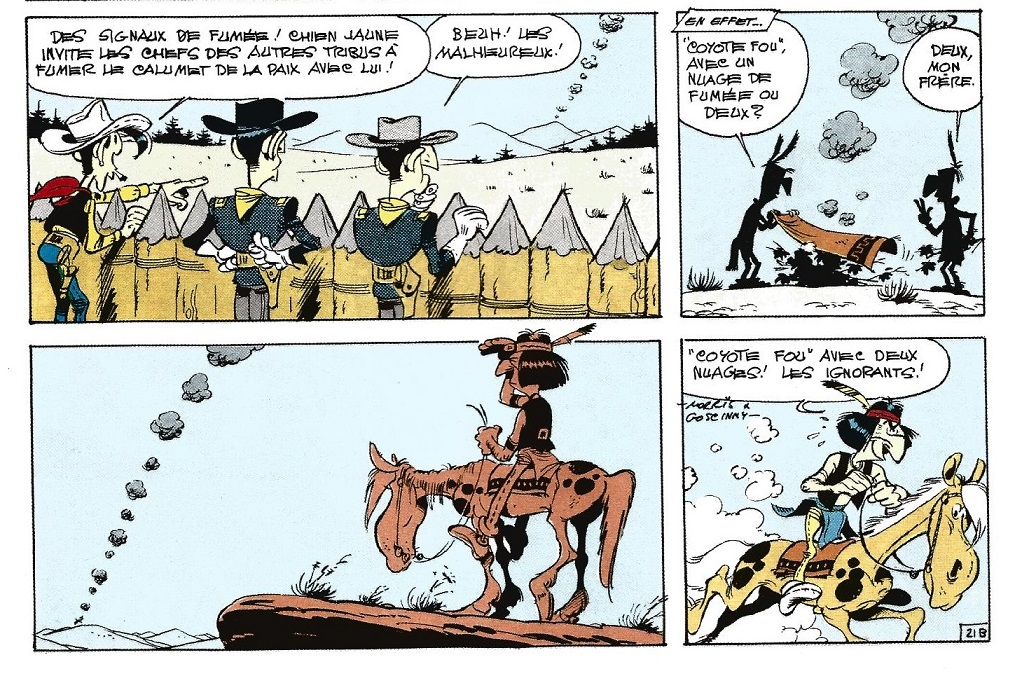
\includegraphics[scale=0.8]{LP_TraitementSignal/Codage_LuckyLuke.jpg}
\end{center}
\textcolor{green}{signal :} (ref Taillet p674) Variation temporelle ou spatiale d'une quantité physique mesurable (tension, force, lumière, ...) portant une information.\\
\textcolor{green}{Traitement du signal :} Transformation d'un signal reçu par un récepteur pour en retirer l'information transmise initialement par un émetteur. Ex : si un observateur cherche à analyser la lumière émise par une étoile (\textcolor{green}{signal}) à travers l'atmosphère, il doit se séparer de celle émise par l'atmosphère (\textcolor{green}{bruit}) par différents moyen (filtrage par exemple).

\section{Représentation des signaux}

\subsection{Types de signaux}
Signaux analogiques vs numériques.\\
Spectre d'énergie d'un signal cf Cottet.\\
\subsection{Décomposition Fourier}
Tout signal peut se décomposer comme une série de signaux sinusoïdaux.\\
Propriétés TF.
\subsection{Echantillonnage}
Mettre Shannon, repliement de spectre (effet de fenêtrage)

\section{Traitement d'un signal}

\subsection{Filtrage, fonction de transfert}
A voir si généralité ou si étude d'un filtre en particulier. Peut-être reprendre leçon de Vincent.
\subsection{Application à la détection synchrone}
\textcolor{blue}{Manip : mesure d'une impédance par détection synchrone}

\subsection{Modulation/démodulation}

\subsection{FFT}

\end{reportBlock}